\documentclass[letterpaper, 10 pt, proceedings]{ieeetran}
\usepackage{amsmath}
\usepackage[margin=.75in]{geometry}
\usepackage{enumitem}
\usepackage{float}
\usepackage{graphicx} % Required for inserting images
\usepackage{helvet}
\usepackage{hyperref}
\usepackage{listings}
\usepackage{mathptmx}
\usepackage{nameref}
\usepackage{pgfplots}
\usepackage{placeins}
\usepackage{subcaption}
\usepackage{titlesec}
\usepackage{wrapfig}
\renewcommand{\familydefault}{\sfdefault}
\graphicspath{{./figures/}}

%\titlespacing*{\section}{0pt}{0.5\baselineskip}{0.25\baselineskip}
%\titlespacing*{\subsection}{0pt}{0.5\baselineskip}{0.25\baselineskip}
%\titlespacing*{\subsubsection}{0pt}{0.5\baselineskip}{0.25\baselineskip}


% Abstract
% Introduction: The goals of the project, the motivation, and the approach used.
% Background: Summary of important concepts and related previous work (with citations).
% Methods: Detailed description of the methods used, including equations, algorithms, rules, etc. and a justification for the approach.
% Results: Description and discussion of results, with figures, tables, etc.
% Conclusion: Summary of accomplishments, challenges and open issues.
% Bibliography: Full list of all papers cited in the report in paper, consistent format




\title{Exploring Stock Market Strategies with Risk and Influence with Complex Networks}
\author{Rachael Judy, Connor Klein, Josh Smith}
\date{21 April 2024}

\begin{document}
	\pgfplotsset{compat=1.18}
	\setlist[itemize]{noitemsep}
	\setlist[enumerate]{noitemsep}
	
	\maketitle

	\begin{abstract}
		This project explores the impact of risk strategies in a complex network of brokers, simulating the stock market over different intervals. It shows how some risk strategies can perform well over typical behavior of the market while others benefit from sudden volatile events. It also explores how influence of broker's friends on the risk assessment can affect the portfolio value over time. 
	\end{abstract}

%	\thanks{This work was contributed by }

	\section{Introduction}\label{sec:intro}
	% Introduction: The goals of the project, the motivation, and the approach used.
	This project was designed with the objective of exploring the impact of risk as defined by a power law distribution and networked brokers in the context of neighbor influence on the brokers' portfolio values over different trading intervals. Economic markets are volatile and have been shown to contain many fat-tailed and power law distributions, such as in growth rates and stock returns \cite{gabix_powerlaws}. Many different models of the market have been created to explore these behaviors, and data is readily available to examine the impacts of different strategies and inter-dependencies on the market. Scholars have examined risk and risk aversion, explored modeling the market as a network of stocks or brokers, attempted to classify and group the networks, and attempted to design models of crashes that resemble the real world. This project combines the study of risk in psychology with the fat tailed distribution of network connections and the volatility of black swan \cite{taleb_antifragile} events to evaluate market broker strategies to maximize portfolio value over typical events and through drastic changes in the market.
	
	\section{Background}\label{sec:background}
	% Background: Summary of important concepts and related previous work (with citations).
	This topic has been explored from a variety of perspectives. Most work has been divided into exploring financial markets in terms of complex networks, looking at individuals' perspective on risk, and running case studies with different clustering and strategies in the market. The work in complex networks creates networks with either brokers or stocks at nodes \cite{kulmann_marketscomplexsystems,dimaggio_relevancebrokernetworks}. To create the edges, they have explored the diffusion of information \cite{dimaggio_relevancebrokernetworks}, spread of first and rebound shocks \cite{gai_contagion}, and correlation and mutual information of different stocks \cite{li_correlation, fiedor_networksmutualinformationrate}. This study models the market with brokers at the nodes with influence connecting the brokers. 
	
	Further, several models for risk were presented. This involved quantifying the risk with the Chen, Roll, and Ross factors \cite{cooper_realinvestmentandrisk} to predict economic activity, assessing the importance of the distribution of risk aversion in the volatility of returns \cite{lansing_riskaversion}, and highlighted the importance of dividends in quantifying the risk level of stocks. These models provide a basis for developing a model of portfolio risk.
	
	Based on the ideas presented in Taleb's book \cite{taleb_antifragile}, it has been suggested that some strategies which perform best over typical market moves may not be optimal during sudden volatile events, which characterize the stock market. The idea that these strategies based on risk with the input on risk assessment from neighbors could be what differentiates the quality of the strategies.
	
	
	\section{Methods}\label{sec:methods}
	% Methods: Detailed description of the methods used, including equations, algorithms, rules, etc. and a justification for the approach.
	The exploration of the market was designed as a simulation to be run over various time intervals for interconnected brokers that can influence one another and preferred risk levels. This included creating 100 brokers each with a preferred risk level and a number of friends sampled from a power law distribution. The friends also provided their assessment of risk for a given stock which was considered by the broker in their personal assessment. Data for every day in the interval was fed into the simulation, allowing brokers, in a random order, to buy or sell stocks to maintain their preferred level of risk. For interpretation of results, the brokers' indices correspond to the level of preferred risk. 
	
	\subsection{Data Collection and Filtering}\label{subsec:data}
	The available tickers were collected from Yahoo Finance's API, yfinance. This API made requests to Yahoo Finance with a request limit being placed on each IP. Fortunaty, the University of Cincinnati offers multiple CPUs in their computer labs. First, all the valid stock tickers were pulled that contained daily stock information from the time peroid of 2000 to 2020, totally 10,000 individual tickers. \par
	These tickers were filtered to those with the information needed for the risk calculation in section \ref{subsec:risk} and 150 stocks were randomly selected from those options to be fed into the simulation. For these stocks, if the price data was missing on a specific day, its price was set to be the most recent value from the time series. Further certain values such as dividend rate and estimated earnings per share were available only as single values instead of time series. This creates inaccuracies in our risk calculation as these single values do flucuate over time, however it is a limitation of the API. This data was then stored in a pandas dataframe for quick accessbility by the simulations at runtime.
	

	\subsection{Influence and Friend Selection}\label{subsec:friends}
	The number of friends for each broker was selected with a power law distribution with $\alpha = 3$ and a minimum value of $2$ friends. The set of friends F were selected randomly from a uniform distribution over all the brokers. Each friend started with a set percent $w_i$ of the broker i's risk assessment. Thus, the risk for a stock $s$ was represented with the formula 
	$$R(\text{s}) = (1-\sum\limits_{f\in F} w_f) R_{broker}(\text{s}) + \sum\limits_{f\in \text{F}} w_f R_f(\text{s})$$

	\subsection{Risk Calculation}\label{subsec:risk}
	% TODO:  @Josh insert mathematical model description, equation, and description of individual and portfolio risk calculation
	
	\subsection{Metrics}\label{subsec:metrics}	
	The portfolio value at any point in time was represented as the sum of the liquid money the broker had and the current value of every stock owned by the broker at the given time. Its risk is evaluated as the risk for every stock in the portfolio multiplied by its volume. The portfolio risk was used to quantify the level of risk each broker attempted to maintain while the portfolio value at different times in the interval was used to evaluate the strategy's overall performance.


	\section{Results}\label{sec:results}
	% Results: Description and discussion of results, with figures, tables, etc.
	
	% risk results
	% Hopefully useful thoughts:
	% - possibly include quick overview showing that high risk brokers tend to own few stocks total of higher value while ones in the middle show the more typical lots of stocks, and most conservative end up with less stocks and more liquid - requires figure of money at end, stock quantity to broker, and liquid money to broker
	% - focus in on a point before 2008 and which level of risk broker is doing well in the wealth time series and then who is doing well after the crash ie high risk
	% - examine immediately after crash wealth v in couple years after
	% - for the case of stop_at_stable and not stop_at_stable, highlight differences in just sitting once at the desired risk v holding the desired risk by buying and selling
	%
	\subsection{Broker Tendencies}\label{subsec:tendencies}	
	As mentioned in \ref{sec:methods}, the index at which each Broker is labeled as directly correlates with the relative initial risk compared to other indices. From this, information can be gleaned from figures of metrics vs broker ID and how these metrics relate to the risk adversion of the brokers. Notabily, a few tendencies commonly developed. These are the owership of individual stocks, the owership of total stocks, and the value of liquid assets.\par
	Fig \ref{totalvID} shows that both low risk and high risk Brokers both tend to own few stocks compared to that of their medium-risk Brokers. Additionally this change in total stocks owned appears to have two critical points at which Brokers preference for total stock owership changes. Interestingly enough this not artifically introduced, but further understanding of this tendency can be descibed by the other tendencies. \par

	\begin{figure}[h]
		\centering
		\twocolumn
		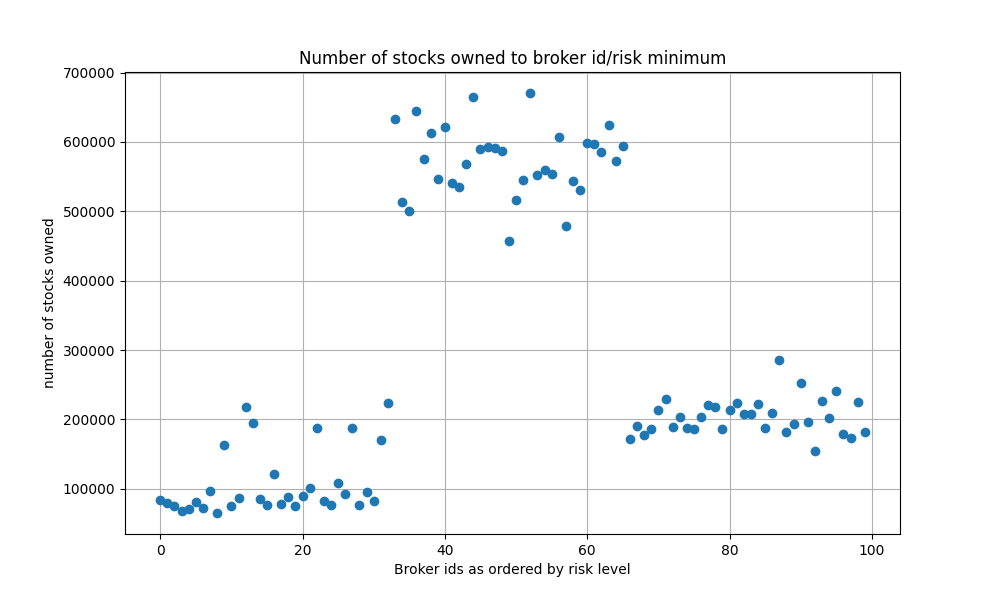
\includegraphics[width=0.4\textwidth]{stocksOwnedToBrokerIds.png}
		\caption{Total number of stocks owned by Broker Id}
		\label{totalvID}
	\end{figure}
	\FloatBarrier

	\begin{figure}[h]
		\centering
		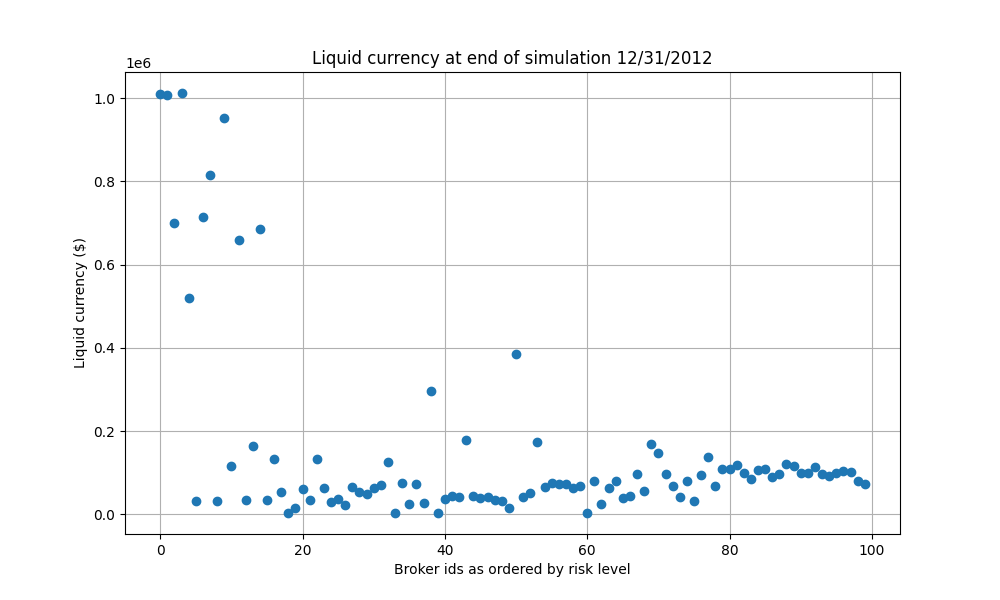
\includegraphics[width=0.4\textwidth]{liquidCurrency.png}
		\caption{Liquid currency vs Broker Id}
		\label{liquidvID}
	\end{figure}
	\FloatBarrier	

	\begin{figure}[h]
		\centering
		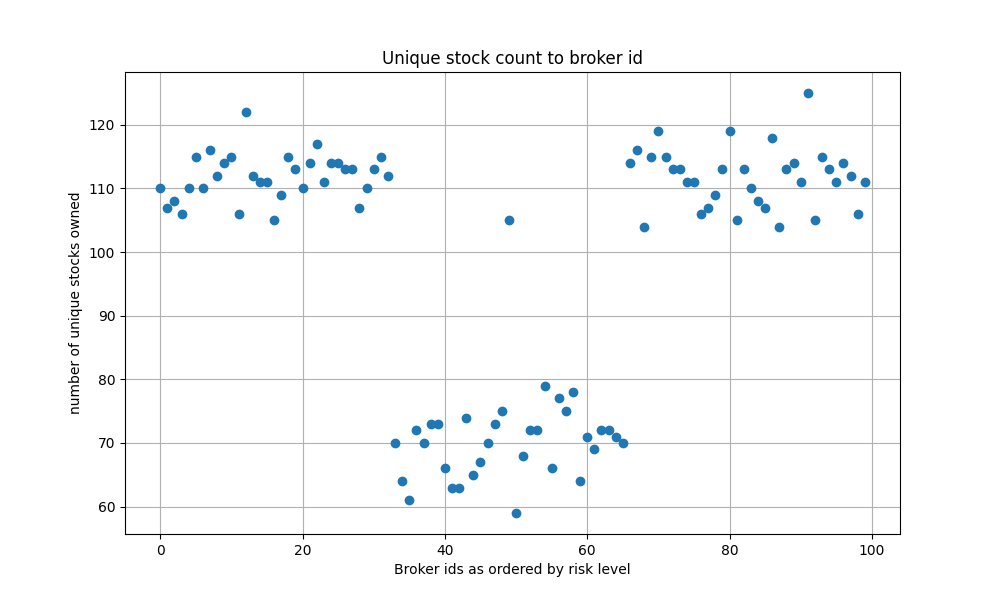
\includegraphics[width=0.4\textwidth]{uniqueStockCountToBrokerIds.png}
		\caption{Uniqie stocks owned by Broker Id}
		\label{uniquevID}
	\end{figure}
	\FloatBarrier

	% here's our figure insertion template
%	\begin{figure}[h]
%		\centering
%		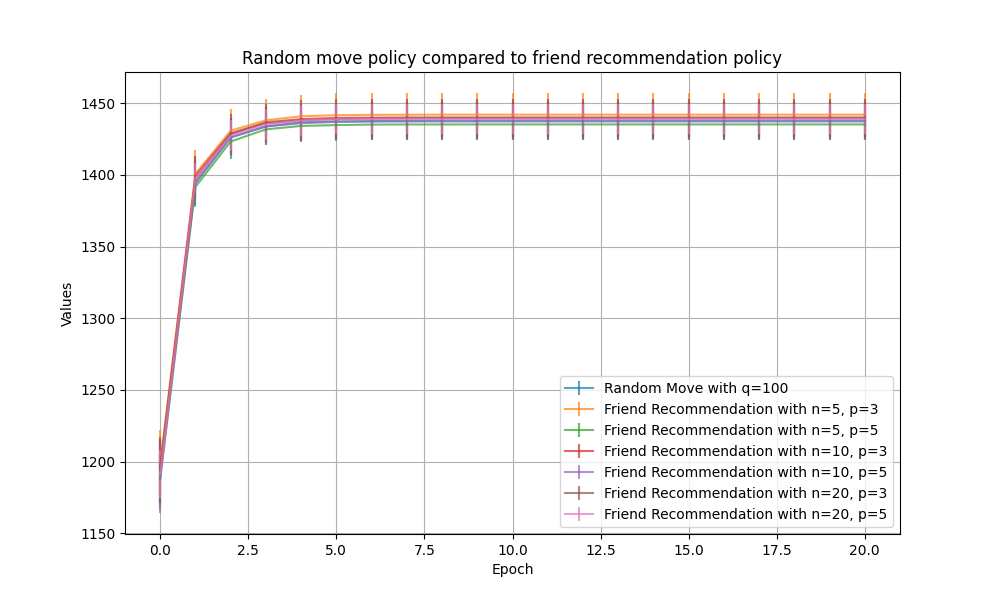
\includegraphics[width=.8\textwidth]{policies01.png}
%		\caption{Time series comparing a random move policy with the social network recommendation policy}
%		\label{p2_ts}
%	\end{figure}	
	
	
	% influence results
	% show mediocre plot of influence to wealth with influence only plots (2 figs)
	% Seems like influence as is feeds into risk incorrectly because the only difference between the broker's assessment is really how much of that stock they own and its value in their portfolio
	% influence would be more relevant if partial information came into play instead of just how risky the broker wanted to be
	
	
	
	\section{Conclusion}\label{sec:conclusion}
	% Conclusion: Summary of accomplishments, challenges and open issues
	This project explored the value of different risk strategies in a simulated market of networked brokers with power law assumptions for risk. It showed ...
	
	\subsection{Future Work}\label{subsec:futurework}
	Given the scope of time for the project, only limited aspects of market strategies could be explored. One open area in which limited advances were made was exploring the impact of the influence of neighbors' assessment of risk on the success of a strategy. Because all neighbors used the same information and formula, except for the accounting of their personal status, the impact of influence could be expanded. Further, the risk assessment would be modified to vary more between brokers based on partial information and stocks without full information available to better represent the real world and better account for the interconnections between stocks. 



	\bibliographystyle{ieeetran}
	\begin{thebibliography}{99}	
		\bibitem{gabix_powerlaws}
		X. Gabaix, “Power laws in economics: an introduction,” \textit{Journal of Economic Perspectives}, vol. 30, no. 1, pp. 185–206, Feb. 2016.
		
		\bibitem{taleb_antifragile}
		N. N. Taleb, Antifragile: Things that gain from disorder. Harlow, England: Penguin Books, 2013.
		
		\bibitem{easley_networkscrowdsmmarkets}
		D. Easley and J. Kleinberg, Networks, crowds, and markets: Reasoning about a highly connected world. Cambridge, England: Cambridge University Press, 2012.
		%- https://www.cs.cornell.edu/home/kleinber/networks-book/, particularly chapters 9-12, 17, 22
		
		\bibitem{thakkar_neuralnets}
		A. Thakkar and K. Chaudhari, “A comprehensive survey on deep neural networks for stock market: The need, challenges, and future directions,” Expert Systems with Applications, vol. 177, p. 114800, Sep. 2021, doi: 10.1016/j.eswa.2021.114800.
		%- https://www.sciencedirect.com/science/article/pii/S0957417421002414
		
		\bibitem{hommes_complexmacroeconomics}
		C. Hommes, “Behavioral and Experimental Macroeconomics and Policy Analysis: A Complex Systems Approach,” Journal of Economic Literature, vol. 59, no. 1, pp. 149–219, Mar. 2021, doi: 10.1257/jel.20191434.
		%- https://pubs.aeaweb.org/doi/pdfplus/10.1257/jel.20191434
		
		\bibitem{tse_networkstocks}
		C. K. Tse, J. Liu, and F. C. M. Lau, “A network perspective of the stock market,” Journal of Empirical Finance, vol. 17, no. 4, pp. 659–667, Sep. 2010, doi: 10.1016/j.jempfin.2010.04.008.
		%- https://www.sciencedirect.com/science/article/pii/S0927539810000368
		
		\bibitem{wikipedia_marketcrashes}
		“List of stock market crashes and bear markets,” Wikipedia. Jan. 24, 2024. Accessed: Feb. 13, 2024. [Online].
		
		\bibitem{kulmann_marketscomplexsystems}
		M. Kuhlmann, "Explaining financial markets in terms of complex systems," \textit{Philosphy of Science}, vol. 81, no. 5, pp. 1117-1130, Dec. 2014. %doi: 10.1086/677699.
		
		\bibitem{dimaggio_relevancebrokernetworks}
		M. Di Maggio, F. Franzoni, A. Kermani, and C. Sommavilla, "The relevance of broker networks for information diffusion in the stock market," \textit{Journal of Financial Economics}, vol. 134, no. 2, pp. 419-446, Nov. 2019. %doi: 10.1016/j.jfineco.2019.04.002. 
		
		
		\bibitem{gai_contagion}
		P. Gai and S. Kapadia, "Contagion in financial networks," \textit{Proceedings of the Royal Society}, vol. 466, no. 2120, pp. 2401–2423, Aug. 2010.
		
		\bibitem{liu_networkperspective}
		C. K. Tse, J. Liu, and F. C. M. Lau, “A network perspective of the stock market,” \textit{Journal of Empirical Finance}, vol. 17, no. 4, pp. 659–667, Sep. 2010. % doi: 10.1016/j.jempfin.2010.04.008.
		
		\bibitem{li_correlation}
		G. Li, A. Zhang, Q. Zhang, D. Wu, and C. Zhan, “Pearson correlation coefficient-based performance enhancement of broad learning system for stock price prediction,” \textit{IEEE Transactions on Circuits and Systems II: Express Briefs}, vol. 69, no. 5, pp. 2413–2417, May 2022. %, doi: 10.1109/TCSII.2022.3160266.
		
		\bibitem{fiedor_networksmutualinformationrate}
		P. Fiedor, “Networks in financial markets based on the mutual information rate,” \textit{Physical Review E}, vol. 89, no. 5, May 2014. % doi: 10.1103/PhysRevE.89.052801.
		
		\bibitem{cooper_realinvestmentandrisk}
		I. Cooper and R. Priestley. "Real investment and risk dynamics," \textit{Journal of Financial Economics}, vol. 101, no. 1, pp. 182-205, July 2011.
		
		\bibitem{lansing_riskaversion}
		K. J. Lansing and S. F. LeRoy, “Risk aversion, investor information and stock market volatility,” \textit{European Economic Review}, vol. 70, pp. 88-107, July 2014. 
		
		\bibitem{risktolerance}
		J. E. Corter and Y. J. Chen, “Do investment risk tolerance attitudes predict portfolio risk?,” \textit{Journal of Business and Psychology}, vol. 20, no. 3, pp. 369-381, 2006.
		
		\bibitem{harmon_economicinterdependence}
		D. Harmon, B. Stacey, Y. Bar-Yam, and Y. Bar-Yam, "Networks of economic market interdependence and systemic risk," New England Complex Systems Institute, Cambridge, MA, Tech. Report 1011.3707, Mar. 2009.
		
		\bibitem{park_complex}
		J. Park, C. H. Cho, and J. W. Lee, "A perspective on complex networks in the stock market," \textit{Frontiers in Physics}, vol. 10, Dec. 2022. %[Online serial] %, doi: 10.3389/fphy.2022.1097489.
		
		\bibitem{baydelli_hierarchicalmarket}
		Y. Y. Baydilli, S. Bayir, and I. Tuker, “A hierarchical view of a national stock market as a complex network,” \textit{Economic Computation \& Economic Cybernetics Studies \& Research}, vol. 51, no. 1, pp. 205–222, Jan. 2017.
		
		
		
	\end{thebibliography}

\end{document}